\documentclass[10pt,a4paper]{article}
\usepackage[margin=23mm]{geometry}
\usepackage[T1]{fontenc}
\usepackage{lmodern,amsmath,amssymb,microtype,booktabs,tabularx,array}
\usepackage{graphicx,xcolor,parskip,caption,fancyhdr}
\usepackage[colorlinks=true,linkcolor=blue!45!black,urlcolor=blue!55!black]{hyperref}
\newcolumntype{Y}{>{\raggedright\arraybackslash}X}
\newcommand{\pdfzero}{\textit{pdf}\textsuperscript{0}}
\newcommand{\fold}{\operatorname{wrap}_{24}}
\renewcommand{\theequation}{S\arabic{equation}}
\renewcommand{\thetable}{S\arabic{table}}
\renewcommand{\thefigure}{S\arabic{figure}}
\captionsetup{font=small,labelfont=bf}
\setlength{\emergencystretch}{2em}
\setlength{\headheight}{14pt}
\pagestyle{fancy}
\fancyhf{}
\fancyhead[L]{\small Supplementary Information}
\fancyhead[R]{\small Dual-oscillator phase model}
\fancyfoot[C]{\thepage}
\raggedbottom
\hypersetup{pdftitle={Supplementary Information: minimal dual-oscillator phase model}}
\begin{document}
\begin{center}
{\Large\bfseries Supplementary Information}\\[5pt]
{\large A minimal dual-oscillator phase model of photoperiod-dependent
transcriptional timing}
\end{center}

This document gives the complete definition of the model described in the
Methods, the analysis that explains its behavior, the fitting procedure,
and an assessment of how well the data constrain its parameters.

\section*{S1. Model definition}
The transcriptional rhythms of the morning (M; sLNv) and evening (E; fifth
sLNv) clock neurons are described by two phases, $\phi_M(t)$ and
$\phi_E(t)$. Each phase advances by $2\pi$ per cycle, and a \textit{tim}
transcriptional peak occurs whenever a phase passes $\pi$. Time $t$ and
photoperiod $P$ are in hours, with zeitgeber time (ZT) 0 at lights-on.
The phases obey
\begin{align}
 \dot\phi_M&=\omega+K\,L(t)\sin(\theta-\phi_M)
              +\kappa\sin(\phi_E-\phi_M)+g_M\,\gamma\,S(t),\label{eq:M}\\
 \dot\phi_E&=\omega+K\,L(t)\sin(\theta-\phi_E)
              -\kappa\sin(\phi_E-\phi_M)-g_E\,\gamma\,S(t),\label{eq:E}
\end{align}
where $\omega=2\pi/24$~rad\,h$^{-1}$ is the intrinsic frequency shared
by both oscillators. The remaining terms describe entrainment by light
(strength $K$), mutual coupling (strength $\kappa$) and a PDF-dependent
drive (strength $\gamma$).

\paragraph{Light and the reference phase.}
Light is a square wave, $L(t)=1$ when $(t\bmod24)<P$ and $0$ otherwise.
In the light, both oscillators are attracted toward a reference phase
\begin{equation}
 \theta(t)=\omega t+\pi-\omega B(P),\label{eq:theta}
\end{equation}
which passes $\pi$ at ZT $B(P)$. The reference peak time $B(P)$ depends on
photoperiod through
\begin{align}
 P_c&=\min(P,15\,\mathrm{h}),\qquad
 x=\max(0,P_c-9\,\mathrm{h}),\qquad
 F(P)=\frac{x^2}{x^2+h_P^2},\label{eq:activation}\\
 B(P)&=\max(P_f,P_c)+\lambda_s+(\lambda-\lambda_s)F(P).\label{eq:B}
\end{align}
The activation function $F(P)$ is zero up to 9~h of light and rises
toward 1 on longer days, with half-activation scale $h_P$. For
photoperiods up to $P_f$ the reference peaks at the fixed time
$P_f+\lambda_s$; between $P_f$ and 9~h it follows lights-off by
$\lambda_s$; above 9~h its delay after lights-off grows from $\lambda_s$
toward $\lambda$; and beyond 15~h it no longer changes. With the values
$P_f=7$~h, $\lambda_s=1$~h and $h_P=1$~h used throughout,
Eq.~\eqref{eq:B} reduces to the form given in the Methods,
$B(P)=\max(8,P_c+1)+(\lambda-1)F(P)$.

\paragraph{PDF-dependent drive.}
The drive is
\begin{equation}
 S(t)=L(t)\max(0,\cos\theta)F(P).\label{eq:drive}
\end{equation}
It acts only in the light, only during the half of the reference cycle
centered 12~h before the reference peak, and only at photoperiods longer
than 9~h. It advances M and delays E with the same strength $\gamma$.
$S(t)$ is an effective description of the action of PDF signaling on
phase; it is not a measurement of PDF release.

\paragraph{Genotypes.}
The flags $(g_M,g_E)$ are $(1,1)$ for wild type, $(0,0)$ for loss of PDF,
$(0,1)$ for M-specific loss of the PDF receptor (PDFR) and $(1,0)$ for
E-specific loss of PDFR. All other terms, including the coupling $\kappa$,
are identical in every genotype. The model does not assign the coupling
to a particular molecular mediator.

\begin{table}[!htb]
\centering\small
\begin{tabularx}{\textwidth}{lrllY}
\toprule
Parameter & Value & Units & Status & Role\\
\midrule
$\omega$ & $2\pi/24$ & rad/h & Fixed & Intrinsic frequency\\
$K$ & 0.0729 & rad/h & Fitted & Strength of light entrainment\\
$\gamma$ & 0.1082 & rad/h & Fitted & Strength of PDF-dependent drive\\
$\kappa$ & 0.00622 & rad/h & Fitted & Strength of M--E coupling\\
$\lambda$ & 3.009 & h & Fitted & Delay of reference peak after lights-off on long days\\
$P_f$ & 7 & h & Fixed & Photoperiod below which the reference peak is constant\\
$\lambda_s$ & 1 & h & Fixed & Delay of reference peak after lights-off on short days\\
$h_P$ & 1 & h & Fixed & Half-activation scale of $F$\\
-- & 9 & h & Fixed & Photoperiod at which $F$ and the drive switch on\\
-- & 15 & h & Fixed & Photoperiod beyond which timing saturates\\
\bottomrule
\end{tabularx}
\caption{Model parameters. Four parameters were fitted (Section S3). The
fixed constants were chosen from the measured peak times, which are at
ZT~8 under 4- and 6-h photoperiods, coincide through 9~h, and saturate
beyond 15~h; the sensitivity of the fit to $P_f$, $\lambda_s$ and $h_P$
is examined in Section S6.}
\label{tab:parameters}
\end{table}

\section*{S2. Analysis: mean phase, phase difference and darkness}
The behavior of the model is clearest in terms of the mean phase
$m=(\phi_M+\phi_E)/2$ and the phase difference $\delta=\phi_E-\phi_M$.
Adding and subtracting Eqs.~\eqref{eq:M} and \eqref{eq:E} gives, without
approximation,
\begin{align}
 \dot m&=\omega+K\,L\sin(\theta-m)\cos(\delta/2)
                      +(g_M-g_E)\,\gamma S/2,\label{eq:mean}\\
 \dot\delta&=-2K\,L\cos(\theta-m)\sin(\delta/2)
                      -2\kappa\sin\delta-(g_M+g_E)\,\gamma S.\label{eq:gap}
\end{align}

\paragraph{Wild type.}
With $g_M=g_E=1$ the PDF-dependent drive cancels from
Eq.~\eqref{eq:mean}. The offset of the mean phase from the reference,
$u=m-\theta$, then obeys
\begin{equation}
 \dot u=-K\,L\sin u\cos(\delta/2),
\end{equation}
so that $u=0$ is an attracting solution whenever $|\delta|<\pi$: under
repeated light--dark cycles the mean phase locks to the reference. On
this solution the phase difference follows
\begin{equation}
 \dot\delta=-2K\,L\sin(\delta/2)-2\kappa\sin\delta-2\gamma S.
 \label{eq:wtgap}
\end{equation}
The first two terms pull $\delta$ toward zero and the third pushes it
away. The reference therefore sets when the two cell groups peak on
average, while the M--E gap is set by competition between the
PDF-dependent drive ($\gamma$) and the two restoring influences, light
($K$) and coupling ($\kappa$). Because E peaks after M, a positive
E-minus-M peak-time gap corresponds to negative $\delta$. All gaps
reported here are differences between actual peak times, not values of
$\delta/\omega$.

\paragraph{Mutants.}
Without PDF ($g_M=g_E=0$) the drive vanishes from both equations,
$\delta=0$ is the attracting solution, and M and E peak together at the
reference peak time $B(P)$. When PDFR is removed from only one cell
group, the drive acts on the other alone: the gap is smaller than in
wild type, and the drive no longer cancels from Eq.~\eqref{eq:mean}, so
the mean phase shifts as well.

\paragraph{Constant darkness.}
In darkness $L=S=0$, and Eqs.~\eqref{eq:mean}--\eqref{eq:gap} become
\begin{equation}
 \dot m=\omega,\qquad
 \dot\delta=-2\kappa\sin\delta,\qquad
 \tan\frac{\delta(t)}{2}
 =\tan\frac{\delta(t_0)}{2}\,e^{-2\kappa(t-t_0)}.
\end{equation}
Both oscillators free-run at the intrinsic frequency while the coupling
closes the gap, with time constant $1/(2\kappa)=80.4$~h for small gaps at
the fitted $\kappa$. Without coupling the gap present at the last
lights-off would persist unchanged.

\paragraph{One peak per day.}
Because every interaction term in Eqs.~\eqref{eq:M}--\eqref{eq:E} is
bounded, both phase velocities satisfy
\begin{equation}
 \dot\phi_i\geq\omega-K-\gamma-\kappa.\label{eq:bound}
\end{equation}
For the fitted parameters the right-hand side is 0.074~rad\,h$^{-1}$,
which is positive. Each phase therefore always advances and cannot
reverse to produce a second peak within a cycle. Fits were restricted to
parameters satisfying $K+\gamma+\kappa<\omega$; Section S7 examines the
effect of this restriction.

\section*{S3. Experimental targets and fitting}
\paragraph{Wild-type targets.}
Peak times were estimated from 10,000 paired, stratified bootstrap
resamples of the 20 brains at each ZT, with M and E resampled together.
The bootstrap mean M and E peak times at 11 photoperiods (4, 6, 9, 10,
11, 12, 13, 14, 15, 18 and 20~h of light; Table~\ref{tab:wt}) were the
fitting targets. For each photoperiod, the covariance of the two peak
estimates was reconstructed from the bootstrap standard deviations of the
M peak, the E peak and their difference,
\begin{equation}
 C_P=
 \begin{pmatrix}
 \sigma_M^2 & (\sigma_M^2+\sigma_E^2-\sigma_{\rm gap}^2)/2\\
 (\sigma_M^2+\sigma_E^2-\sigma_{\rm gap}^2)/2 & \sigma_E^2
 \end{pmatrix}
 +\frac{(1\,\mathrm{h})^2}{12}I.
\end{equation}
The last term is the variance of a uniform distribution over the 1-h
sampling interval and prevents peaks with near-zero bootstrap spread from
dominating the fit. Writing $C_P=A_PA_P^{\mathsf T}$, the weighted
residual at photoperiod $P$ is
$r_P=A_P^{-1}\fold(\widehat{\mathbf y}_P-\mathbf y_P)$, where
$\mathbf y_P$ and $\widehat{\mathbf y}_P$ are the observed and model
M and E peak times and $\fold$ wraps each difference into
$[-12,12)$~h. The M--E gap was not fitted as a separate quantity.

\paragraph{Mutant and darkness targets.}
Mutant targets at 12L:12D (Table~\ref{tab:mutants}) entered with a scale
of 0.5~h. They contribute five residuals: the single shared peak time
for loss of PDF, and the M and E peak times for each receptor-loss
genotype. For a simulated transfer from 12L:12D to constant darkness
(DD), with $G_d$ the E-minus-M peak-time gap on day $d$,
\begin{equation}
 r_{\rm DD}=
 \left(
 \frac{G_1-3.1\,\mathrm{h}}{0.75\,\mathrm{h}},\,
 \frac{\max(0,|G_4|-1\,\mathrm{h})}{0.5\,\mathrm{h}}
 \right),
\end{equation}
which asks for a gap near 3.1~h on the first day and below 1~h on the
fourth. The mutant and darkness scales express how closely these
qualitative results should be matched; they are not measured standard
deviations.

\paragraph{Objective.}
The fitted parameters $(K,\lambda,\gamma,\kappa)$ minimized
\begin{equation}
 J=\sum_P\|r_P\|^2+\|r_{\rm mut}\|^2
                         +\|r_{\rm DD}\|^2+\|r_{\rm lock}\|^2.
\end{equation}
The last term penalizes solutions that do not settle onto a stable 24-h
rhythm. It comprises, over the final two simulated days, 10 times the
day-to-day change in each peak time (in hours) and, for each oscillator,
100 times the deviation from one rotation per day and from one peak per
day. It is negligible at the fitted solution (Section S5).

\paragraph{Optimization.}
We used bounded nonlinear least squares
(\texttt{scipy.optimize.least\_squares}) from multiple starting points,
with bounds $K\in[0.02,0.5]$, $\gamma\in[0,0.8]$ and
$\kappa\in[0.001,0.08]$~rad\,h$^{-1}$, $\lambda\in[0,6]$~h, and the
restriction $K+\gamma+\kappa<\omega$.

\section*{S4. Numerical methods and checks}
Equations~\eqref{eq:M}--\eqref{eq:E} were integrated with the adaptive
LSODA solver (\texttt{scipy.integrate.odeint}; relative and absolute
tolerances $2\times10^{-7}$ and $10^{-9}$; maximum step 1~h) from
$\phi_M=\phi_E=\pi$. Lights-on and lights-off times were supplied as
integration breakpoints. Peak times were obtained by interpolating the
times at which each phase crossed $\pi$ on a 0.1-h output grid. During
fitting, simulations ran for 40 days and the last two days were used;
all reported predictions were read out after 60 days.

Three checks support the reported values. First, an independent
implementation that integrates Eqs.~\eqref{eq:mean}--\eqref{eq:gap}
with tighter tolerances agreed with the direct integration to within
0.005~h for peak times under light--dark cycles and 0.006~h for gaps in
darkness. Second, 80-day simulations from three initial phase pairs,
$(\pi,\pi)$, $(0,1.7)$ and $(2.2,5.4)$, for wild type at every
photoperiod from 4 to 20~h and for the three mutant genotypes at 12L:12D
all converged to the same rhythm: peak times differed by at most
0.004~h between initial conditions. Third, in every one of these
simulations each oscillator produced exactly one peak per day, completed
one rotation per day to within 0.005 cycles, and showed a day-to-day
change in peak time of at most 0.004~h.

Model predictions are for the settled rhythm. Experimental measurements
were made after a finite number of days in each light--dark cycle, and
the phases at the start of each experiment are not known, so the
simulations do not reproduce the entrainment history of the animals.

\section*{S5. Model fit}
The fitted model has $J=6.12$, of which 4.78 comes from the 22 wild-type
peak times, 1.05 from the mutant targets, 0.29 from the darkness targets
and less than 0.001 from the locking term. The unweighted
root-mean-square error over the 22 wild-type peak times is 0.229~h
(Fig.~\ref{fig:fit}a,b; Table~\ref{tab:wt}).

\begin{figure}[!htb]
\centering
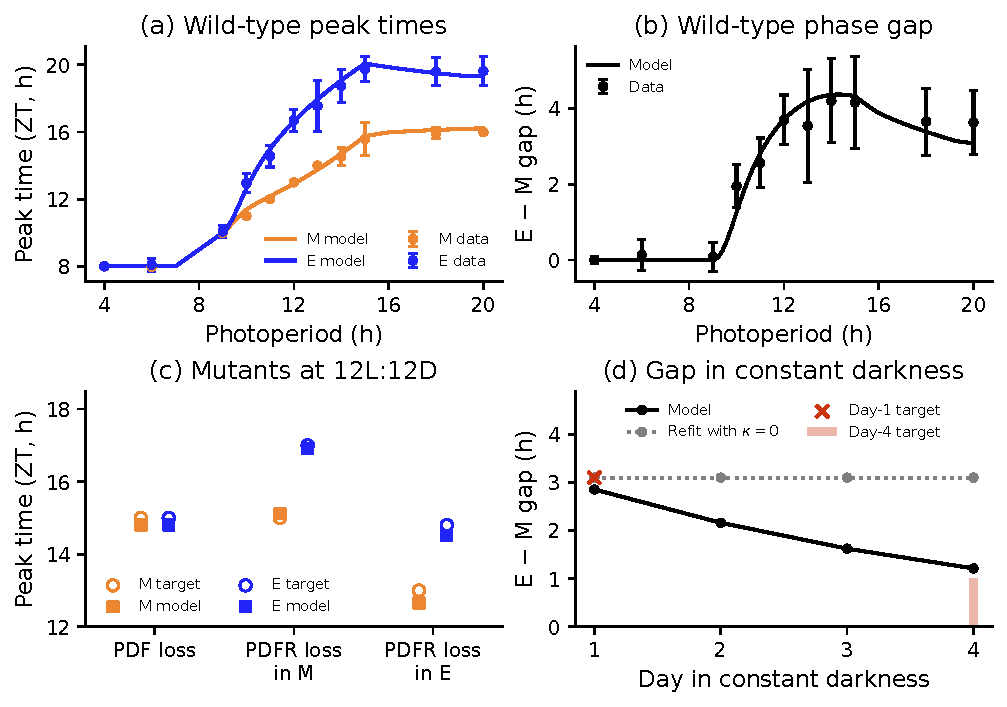
\includegraphics[width=0.92\textwidth]{figure/supplementary/model_fit.pdf}
\caption{Model fit. (a) Wild-type M and E peak times and (b) their
difference as a function of photoperiod. Points and error bars are
bootstrap means and standard deviations; lines are model predictions.
The gap in (b) is derived from the paired peak times and was not fitted
separately. (c) Peak times of the three mutant genotypes at 12L:12D.
(d) E-minus-M gap on successive days after transfer from 12L:12D to
constant darkness, for the fitted model and for a refit without coupling
($\kappa=0$). The cross and the shaded bar mark the day-1 and day-4
targets.}
\label{fig:fit}
\end{figure}

\begin{table}[!htb]
\centering\small
\begin{tabular}{rrrrrrr}
\toprule
 & \multicolumn{2}{c}{M peak (ZT, h)} & \multicolumn{2}{c}{E peak (ZT, h)}
 & \multicolumn{2}{c}{E $-$ M gap (h)}\\
\cmidrule(lr){2-3}\cmidrule(lr){4-5}\cmidrule(lr){6-7}
Photoperiod (h) & Data & Model & Data & Model & Data & Model\\
\midrule
4 & 8.00 $\pm$ 0.00 & 8.00 & 8.00 $\pm$ 0.09 & 8.00 & 0.00 & 0.00 \\
6 & 7.97 $\pm$ 0.19 & 8.00 & 8.10 $\pm$ 0.38 & 8.00 & 0.13 & 0.00 \\
9 & 10.00 $\pm$ 0.03 & 10.00 & 10.08 $\pm$ 0.37 & 10.00 & 0.08 & 0.00 \\
10 & 11.00 $\pm$ 0.00 & 11.37 & 12.95 $\pm$ 0.58 & 12.63 & 1.95 & 1.26 \\
11 & 12.00 $\pm$ 0.01 & 12.17 & 14.57 $\pm$ 0.65 & 15.00 & 2.57 & 2.82 \\
12 & 13.00 $\pm$ 0.04 & 12.92 & 16.70 $\pm$ 0.66 & 16.63 & 3.70 & 3.71 \\
13 & 14.00 $\pm$ 0.01 & 13.76 & 17.54 $\pm$ 1.49 & 17.94 & 3.54 & 4.18 \\
14 & 14.54 $\pm$ 0.51 & 14.70 & 18.74 $\pm$ 0.98 & 19.07 & 4.21 & 4.37 \\
15 & 15.59 $\pm$ 0.96 & 15.74 & 19.75 $\pm$ 0.73 & 20.07 & 4.16 & 4.33 \\
18 & 15.93 $\pm$ 0.32 & 16.11 & 19.59 $\pm$ 0.82 & 19.51 & 3.66 & 3.40 \\
20 & 15.99 $\pm$ 0.12 & 16.22 & 19.62 $\pm$ 0.84 & 19.30 & 3.63 & 3.08 \\
\bottomrule
\end{tabular}
\caption{Wild-type peak times. Data are bootstrap means $\pm$ standard
deviations; the data gap is the bootstrap mean of the paired difference.}
\label{tab:wt}
\end{table}

\begin{table}[!htb]
\centering\small
\begin{tabular}{lrrrr}
\toprule
Genotype (12L:12D) & M target & E target & M model & E model\\
\midrule
Loss of PDF (\pdfzero{}) & 15.0 & 15.0 & 14.81 & 14.81 \\
M-specific loss of PDFR & 15.0 & 17.0 & 15.12 & 16.92 \\
E-specific loss of PDFR & 13.0 & 14.8 & 12.65 & 14.51 \\
\bottomrule
\end{tabular}
\caption{Mutant peak times in ZT hours. Targets are rounded summaries of
the experimental peak times.}
\label{tab:mutants}
\end{table}

\paragraph{Mutants.}
The model reproduces the three mutant conditions to within 0.35~h
(Fig.~\ref{fig:fit}c; Table~\ref{tab:mutants}). Loss of PDF places both
peaks at the reference peak time; loss of PDFR in one cell group moves
that group to near the reference peak time and shifts the other by only
about 0.3~h.

\paragraph{Constant darkness and the role of coupling.}
After transfer from 12L:12D to darkness the model gap is 2.85, 2.16, 1.62
and 1.21~h on days 1 to 4 (Fig.~\ref{fig:fit}d). The gap therefore closes
progressively, but on day 4 it remains 0.2~h above the 1-h target. When
the coupling is removed ($\kappa=0$) and the model is refitted (with
$h_P$ also free), the gap
stays at 3.1~h on all four days and the objective rises from 6.12 to
29.53, with 17.5 of the total from the darkness targets; the wild-type
root-mean-square error also increases, to 0.339~h. The coupling is thus
required to close the gap in darkness.

\paragraph{Leave-one-photoperiod-out refits.}
Refitting the four parameters with each photoperiod omitted in turn, and
predicting the omitted M and E peak times, gave a root-mean-square error
of 0.240~h, close to the 0.229~h of the full fit. The fixed constants and
the mutant and darkness targets were kept in every refit, so this is a
check on the stability of the fit, not an independent estimate of
predictive error.

\section*{S6. Sensitivity to the fixed constants and parameter
identifiability}
\paragraph{Fitting the fixed constants.}
To test the choice of $P_f$, $\lambda_s$ and $h_P$, we fitted them
together with $(K,\lambda,\gamma,\kappa)$, using the same objective and
bounds $P_f\in[4,9]$, $\lambda_s\in[0,4]$ and $h_P\in[0.15,5]$~h. The
best seven-parameter fit found (Table~\ref{tab:seven}) has
$J_{\min}=5.85$ and a wild-type root-mean-square error of 0.213~h,
compared with 6.12 and 0.229~h for the four-parameter model. The fitted
constants are close to the fixed values, and the remaining parameters
change by less than 4\%. The model gap in darkness is essentially
unchanged (2.82 and 1.20~h on days 1 and 4). The rounded constants are
therefore adequate, and all results in the main text use the
four-parameter model.

\begin{table}[!htb]
\centering\small
\begin{tabular}{lrrl}
\toprule
Parameter & Four-parameter model & Seven-parameter fit & Units\\
\midrule
$K$ & 0.0729 & 0.0754 & rad/h\\
$\gamma$ & 0.1082 & 0.1095 & rad/h\\
$\kappa$ & 0.00622 & 0.00621 & rad/h\\
$\lambda$ & 3.009 & 2.927 & h\\
$P_f$ & 7 (fixed) & 7.055 & h\\
$\lambda_s$ & 1 (fixed) & 0.953 & h\\
$h_P$ & 1 (fixed) & 0.906 & h\\
\midrule
$J$ & 6.12 & 5.85 & \\
Wild-type RMSE & 0.229 & 0.213 & h\\
\bottomrule
\end{tabular}
\caption{Effect of fitting the three fixed constants.}
\label{tab:seven}
\end{table}

\paragraph{Profiles.}
To assess how well each parameter is determined, we fixed one of $K$,
$\gamma$, $\kappa$, $h_P$, $P_f$ and $\lambda_s$ at a series of values
and refitted all the others, including $\lambda$, with the same
objective (Fig.~\ref{fig:profiles}). Each profile point was started from
at least three initial guesses, and neighboring solutions were used as
further starting points; in total the profiles comprise 411 fits,
seeded from 18 initial full-model starts, 14 of them drawn from a
Latin-hypercube design. Table~\ref{tab:ranges} lists the range of each
parameter over which the objective stays within 1 of $J_{\min}$. All
solutions within 4 of $J_{\min}$ passed the settling checks of
Section S4.

\begin{table}[!htb]
\centering\small
\begin{tabular}{lrl}
\toprule
Quantity & Range with $J-J_{\min}\leq1$ & Units\\
\midrule
$K$ & 0.048--0.105 & rad/h\\
$\gamma$ & 0.065--0.150 & rad/h\\
$\kappa$ & 0.0049--0.0080 & rad/h\\
$h_P$ & 0.60--1.23 & h\\
$P_f$ & 7.00--7.29 & h\\
$\lambda_s$ & 0.81--1.15 & h\\
\midrule
$\gamma/K$ & 1.35--1.55 & --\\
$P_f+\lambda_s$ & 7.95--8.10 & h\\
\bottomrule
\end{tabular}
\caption{Ranges of each profiled quantity over which the objective
remains within 1 of its minimum. The ranges are read from the sampled
profile points and are descriptive: because the mutant and darkness
scales are not measured uncertainties, $J$ is not a calibrated
likelihood and these are not confidence intervals. The upper limits for
$K$ and $\gamma$ reflect the restriction $K+\gamma+\kappa<\omega$
(Section S7).}
\label{tab:ranges}
\end{table}

\begin{figure}[!htb]
\centering
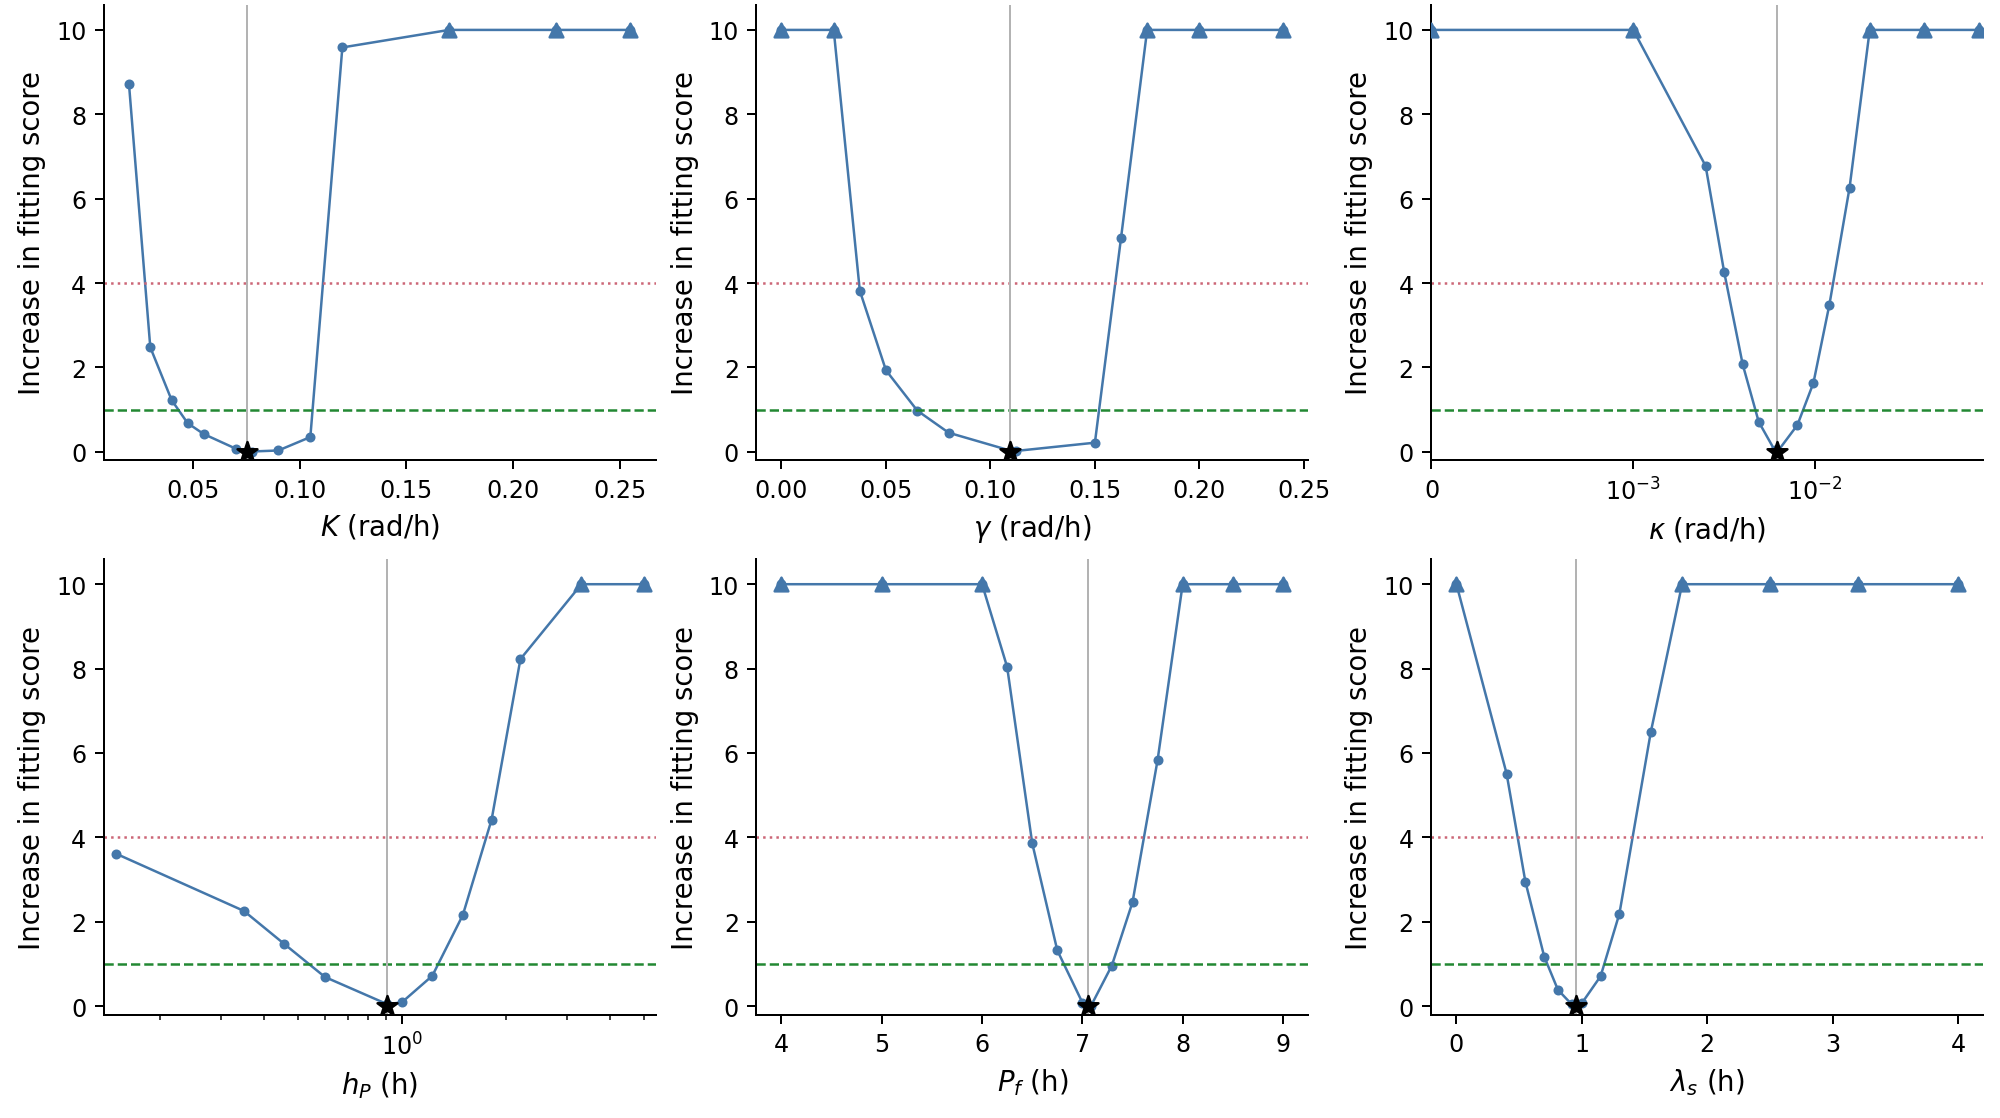
\includegraphics[width=\textwidth]{figure/supplementary/profiles.png}
\caption{Parameter profiles. Each panel shows the increase in the
objective above $J_{\min}$ when one parameter is held fixed and all
others are refitted. The star marks the best fit; dashed and dotted
lines mark increases of 1 and 4. Increases above 10 are drawn at 10
(triangles). The $h_P$ axis is logarithmic; the $\kappa$ axis is linear
near zero and logarithmic above.}
\label{fig:profiles}
\end{figure}

\paragraph{Compensating parameters.}
The coupling $\kappa$ is well determined, because it alone controls the
closing of the gap in darkness; fixing $\kappa=0$ raises the objective
by 23.7. The reference constants $P_f$ and $\lambda_s$ are individually
constrained to within a few tenths of an hour, and their sum, the
short-day peak time, more tightly still. By contrast, $K$ and $\gamma$
can each vary about twofold with little loss of fit, because they
compensate for one another (Fig.~\ref{fig:tradeoffs}): a stronger light
input can be offset by a stronger PDF-dependent drive, as expected from
Eq.~\eqref{eq:wtgap}. A local sensitivity analysis at the best fit gave
a correlation of 0.96 between the estimates of $K$ and $\gamma$ and of
$-0.78$ between $P_f$ and $\lambda_s$. Profiling the ratio $\gamma/K$ and
the sum $P_f+\lambda_s$ directly (Fig.~\ref{fig:combinations}) confirms
that these combinations are determined more tightly than their
components. The half-activation scale $h_P$ is the least constrained
constant: within an increase of 4 its range extends down to the lowest
value tested, 0.15~h. The data therefore fix the balance between the
PDF-dependent drive and light entrainment more firmly than the absolute
strength of either.

\begin{figure}[!htb]
\centering
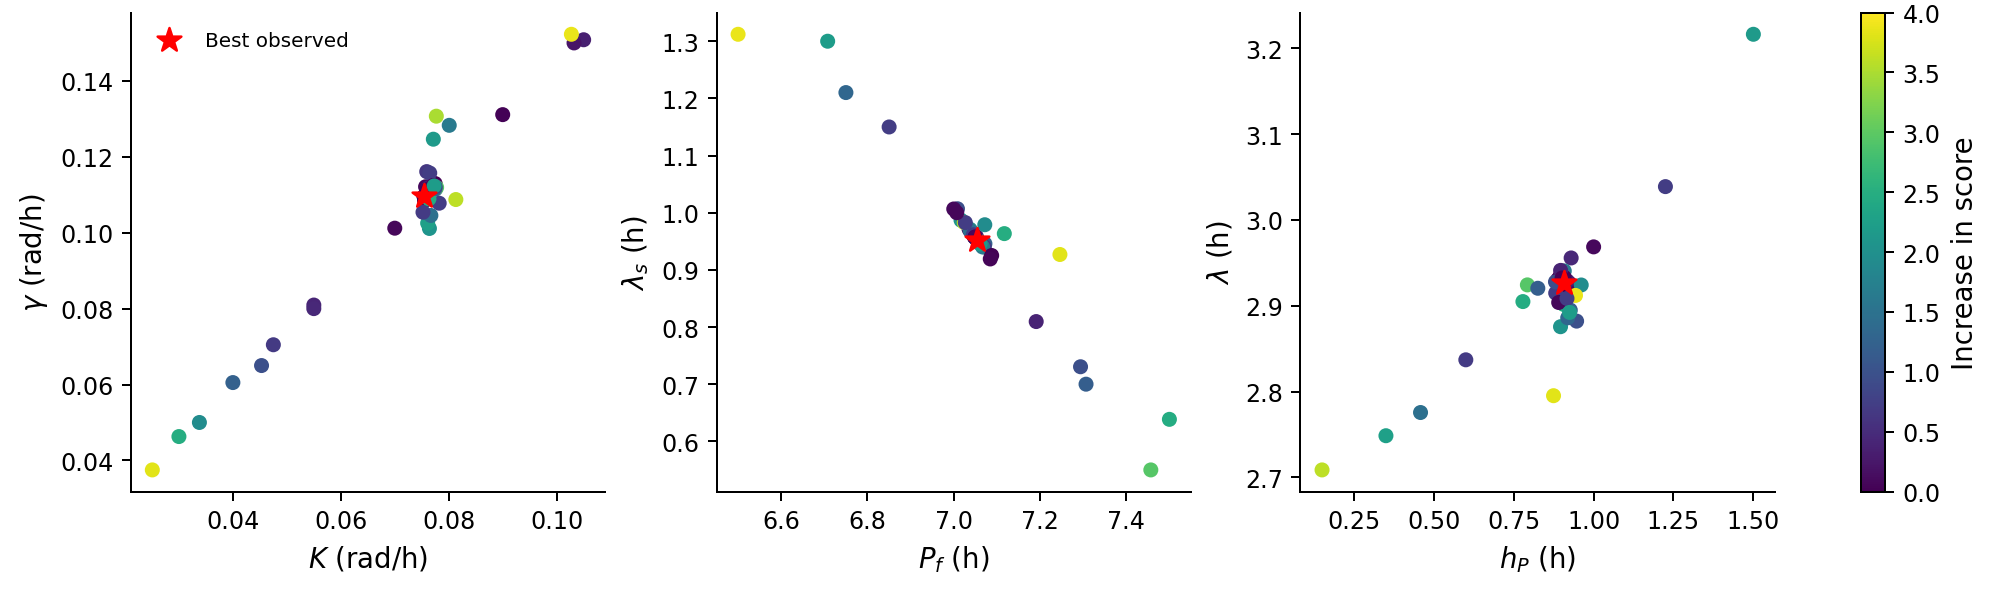
\includegraphics[width=\textwidth]{figure/supplementary/tradeoffs.png}
\caption{Compensation between parameters. Points are the profile
solutions with an objective within 4 of $J_{\min}$, colored by the
increase; the star marks the best fit. The points illustrate the
directions of compensation and are not samples from a probability
distribution.}
\label{fig:tradeoffs}
\end{figure}

\begin{figure}[!htb]
\centering
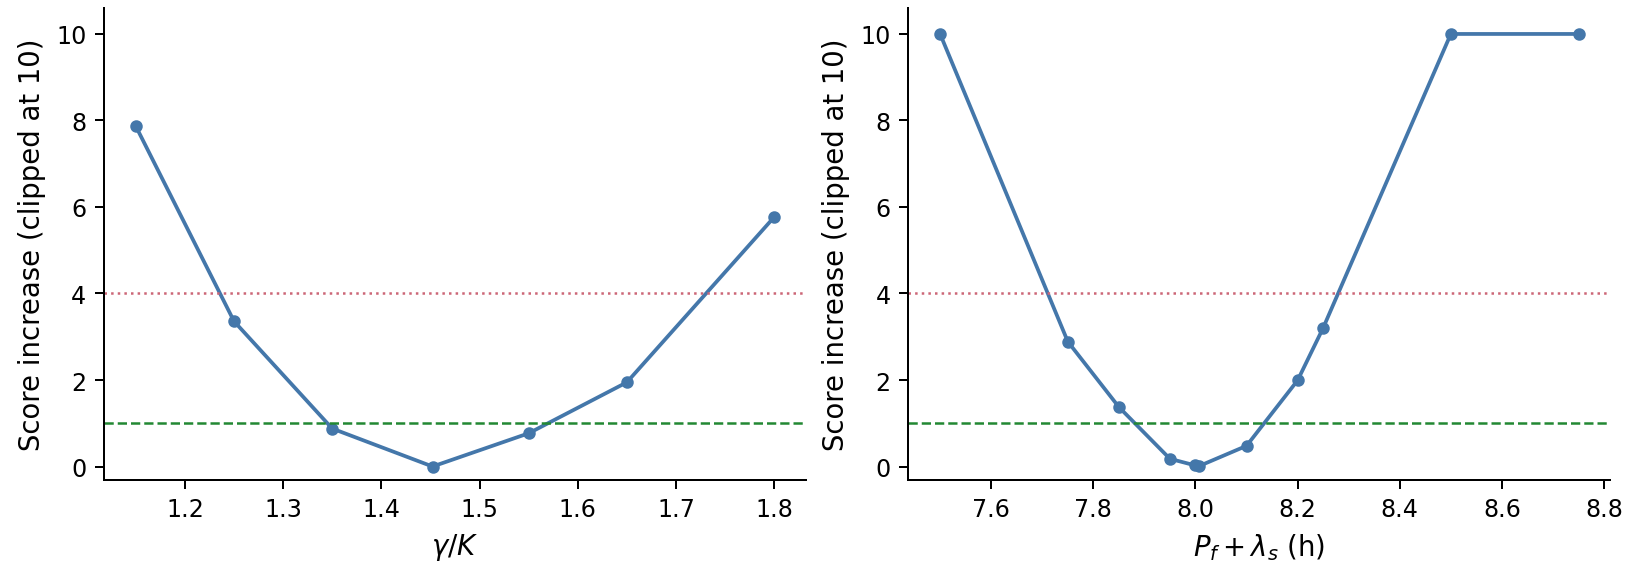
\includegraphics[width=0.85\textwidth]{figure/supplementary/combination_profiles.png}
\caption{Profiles of the ratio $\gamma/K$ and of the sum $P_f+\lambda_s$,
with all other parameters refitted. Dashed and dotted lines mark
increases of 1 and 4; increases above 10 are drawn at 10.}
\label{fig:combinations}
\end{figure}

\section*{S7. Effect of the restriction on parameter strengths}
The restriction $K+\gamma+\kappa<\omega$ guarantees that the phases
always advance (Eq.~\ref{eq:bound}), but it also limits how large $K$
and $\gamma$ can be. To separate this limit from what the data require,
we repeated the fit without the restriction, holding $K$ at larger
values and preventing phase reversal directly by replacing each
right-hand side of Eqs.~\eqref{eq:M}--\eqref{eq:E} with its positive
part, $\max(0,\dot\phi_i)$.

\begin{table}[!htb]
\centering\small
\begin{tabular}{rrrrr}
\toprule
$K$ (rad/h) & $\gamma$ (rad/h) & $\kappa$ (rad/h) & $J$ & $J-J_{\min}$\\
\midrule
0.120 & 0.177 & 0.0061 & 6.29 & 0.44\\
0.170 & 0.264 & 0.0057 & 7.80 & 1.95\\
0.250 & 0.417 & 0.0055 & 11.98 & 6.13\\
0.400 & 0.641 & 0.0039 & 45.41 & 39.56\\
\bottomrule
\end{tabular}
\caption{Best fits with $K$ held fixed and the restriction
$K+\gamma+\kappa<\omega$ removed. All four passed the settling checks of
Section S4.}
\label{tab:domain}
\end{table}

A fit with $K=0.12$~rad\,h$^{-1}$, outside the restricted range, is
almost as good as the best fit, and $\gamma$ again rises with $K$
(Table~\ref{tab:domain}). For $K$ up to 0.25~rad\,h$^{-1}$ the positive
part was never active on the settled rhythm, so these solutions obey
Eqs.~\eqref{eq:M}--\eqref{eq:E} unchanged. The upper ends of the ranges for $K$ and $\gamma$ in
Table~\ref{tab:ranges} are therefore set by the restriction and should
not be read as biological upper limits. Much larger strengths
($K=0.4$~rad\,h$^{-1}$) fit poorly.

\section*{S8. Scope and limitations}
The model shows that three effective influences, light entrainment toward
a common reference, a PDF-dependent drive that separates M and E, and a
weak coupling that draws them together, are sufficient to account for
the settled peak times across photoperiods, their changes in the mutant
genotypes, and the closing of the gap in darkness. Its limitations are
as follows.
\begin{itemize}
\item Photoperiod enters as an input through $F(P)$ and $B(P)$. The
model does not explain how the clock neurons measure day length from
their history of light exposure.
\item The reference phase and the timing of the drive are
phenomenological, and their landmarks (9~h, 15~h, $P_f$, $\lambda_s$ and
$h_P$) were chosen from the same data that were fitted.
\item The strengths $K$ and $\gamma$ are determined mainly through their
ratio (Section S6), so their absolute values should not be interpreted
individually.
\item The model does not address transcriptional amplitudes or waveform
shapes, responses to light pulses, or the absolute phase reached after
several days in darkness, and its gap on the fourth day of darkness
remains slightly above the target.
\end{itemize}
Additional measurements could resolve the compensation between $K$ and
$\gamma$. The recovery of both peak times after a defined phase
perturbation under an unchanged light--dark cycle would constrain $K$
directly; a complete time course of the gap in constant darkness would
constrain $\kappa$ through $\dot\delta=-2\kappa\sin\delta$; and
additional photoperiods between 9 and 11~h would constrain $h_P$.

\paragraph{Code and data availability.}
The model code, fitted parameters, the experimental targets used for
fitting, and the scripts that generate the figures and tables in this
document are available at [repository URL / data availability
statement].
\end{document}
